% begin module compare-linear
\begin{frame}
\ \only<handout:0| -1>{%
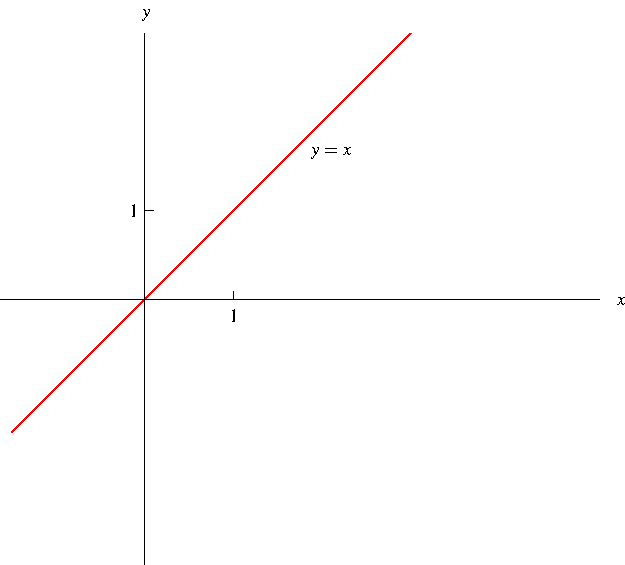
\includegraphics[height=5cm]{../../modules/lines-2d/pictures/01-02-positivea.pdf}%
}%
\only<handout:0| 2>{%
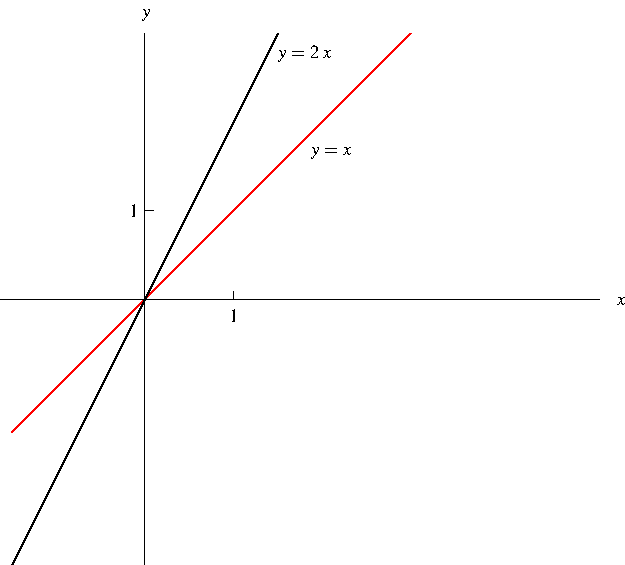
\includegraphics[height=5cm]{../../modules/lines-2d/pictures/01-02-positiveb.pdf}%
}%
\only<handout:0| 3>{%
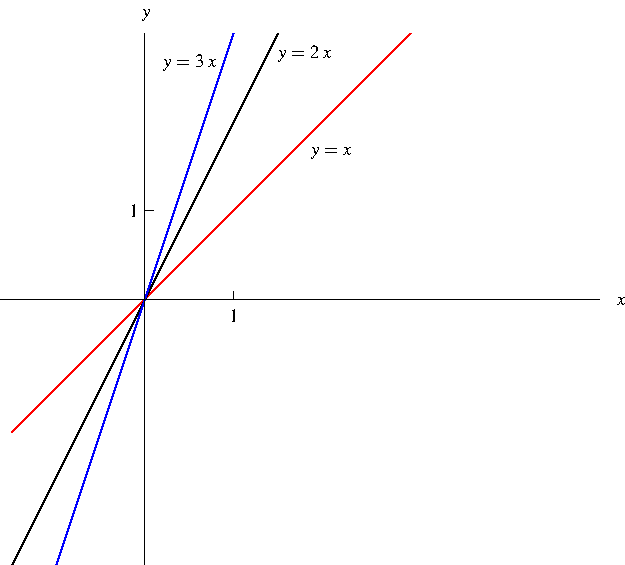
\includegraphics[height=5cm]{../../modules/lines-2d/pictures/01-02-positivec.pdf}%
}%
\only<handout:0| 4>{%
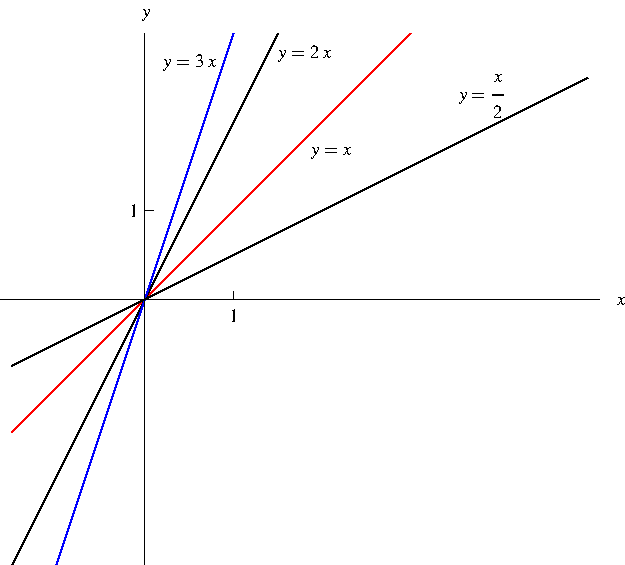
\includegraphics[height=5cm]{../../modules/lines-2d/pictures/01-02-positived.pdf}%
}%
\only<5>{%
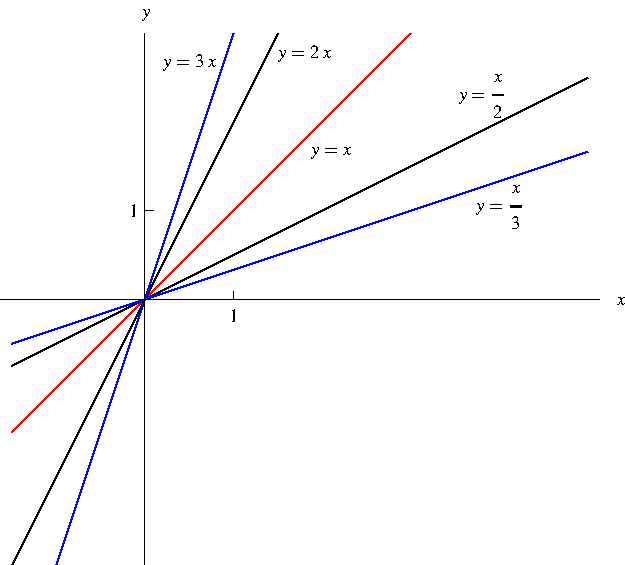
\includegraphics[height=5cm]{../../modules/lines-2d/pictures/01-02-positivee.pdf}%
}%

\begin{itemize}
\item<1->  If two linear functions have positive slopes, the one with the bigger slope increases faster.
\item<2->  $y = 2x$ increases twice as fast as $y = x$.
\item<3->  $y = 3x$ increases three times as fast as $y = x$.
\item<4->  $y = \frac{x}{2}$ increases half as fast as $y = x$.
\item<5->  $y = \frac{x}{3}$ increases one third as fast as $y = x$.
\end{itemize}
\end{frame}

\begin{frame}
\ \only<handout:0| -1>{%
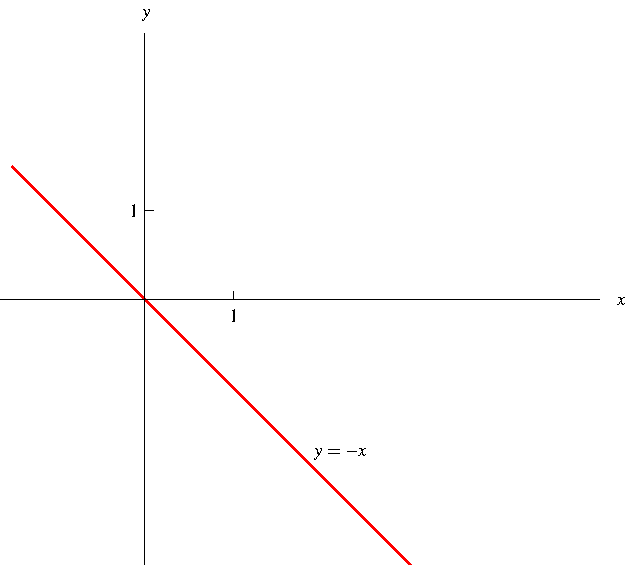
\includegraphics[height=5cm]{precalculus/pictures/01-02-negativea.pdf}%
}%
\only<handout:0| 2>{%
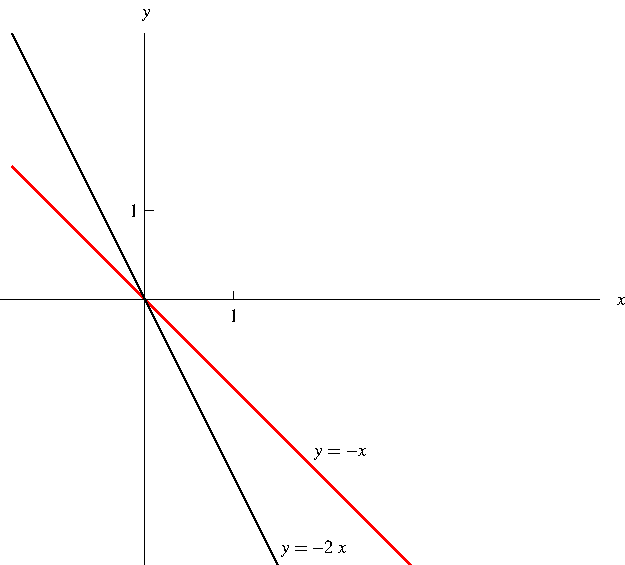
\includegraphics[height=5cm]{precalculus/pictures/01-02-negativeb.pdf}%
}%
\only<handout:0| 3>{%
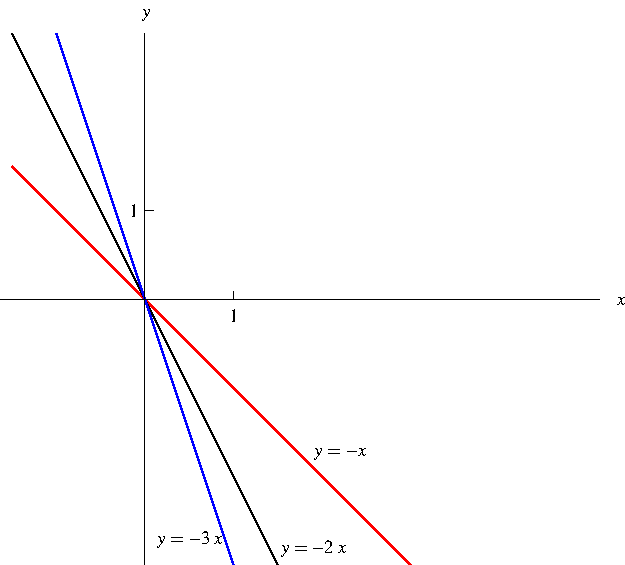
\includegraphics[height=5cm]{precalculus/pictures/01-02-negativec.pdf}%
}%
\only<handout:0| 4>{%
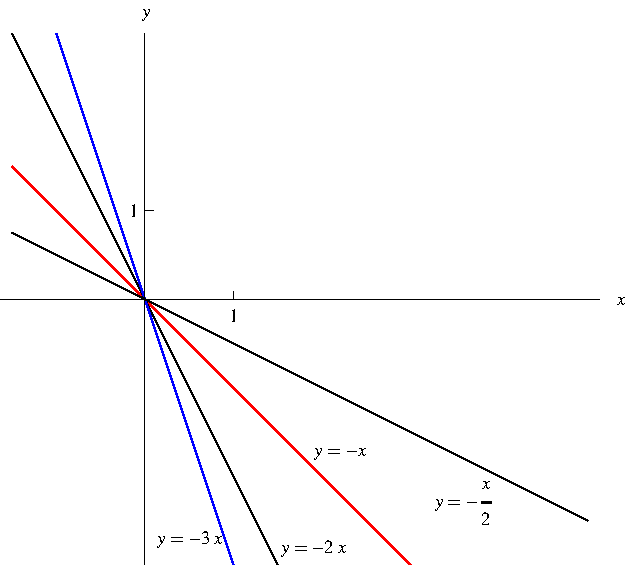
\includegraphics[height=5cm]{precalculus/pictures/01-02-negatived.pdf}%
}%
\only<5>{%
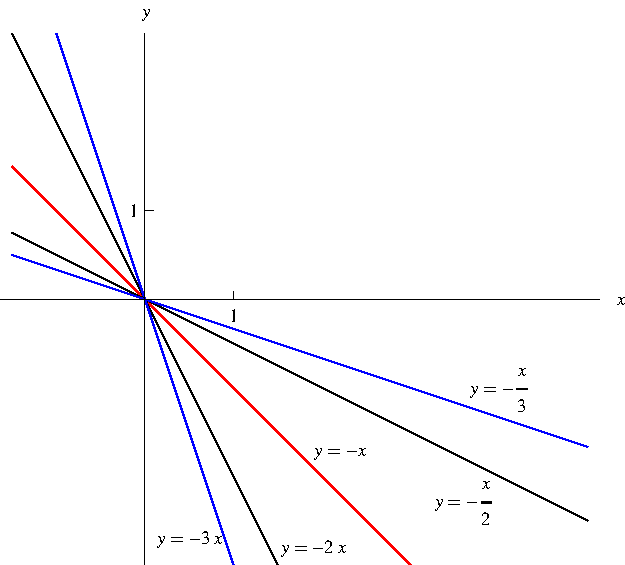
\includegraphics[height=5cm]{precalculus/pictures/01-02-negativee.pdf}%
}%

\begin{itemize}
\item<1->  If two linear functions have negative slopes, the one with the lower slope decreases faster.
\item<2->  $y = -2x$ decreases twice as fast as $y = -x$.
\item<3->  $y = -3x$ decreases three times as fast as $y = -x$.
\item<4->  $y = -\frac{1}{2}x$ decreases half as fast as $y = -x$.
\item<5->  $y = -\frac{1}{3}x$ decreases one third as fast as $y = -x$.
\end{itemize}
\end{frame}
% end module compare-linear
